\documentclass[a4paper, titlepage]{article}
\usepackage{graphicx}
\usepackage{biblatex}
\usepackage{parskip}
\usepackage{listings}
\usepackage{xcolor}
\usepackage{subfig}

\graphicspath{ {./Images/} }

\addbibresource{biblography.bib}
\setcounter{tocdepth}{4}

\title{Analysis Module Documentation}
\author{Adam Rehman, Brandon Cann, Xin Wang \thanks{document compiled by Xin Wang}}
\date{ \today}

\setlength{\parskip}{1em}
\setcounter{tocdepth}{4}
\setcounter{secnumdepth}{4}

\begin{document}
    \maketitle
    \tableofcontents
    \pagebreak
    \section{Introduction}
    \par
    This document will research the theory of analysing a circuit and design the $Analyser$ module.
    The $Analyser$ module will create the matrices required to perform the nodal analysis and, using the 
    matrices, perform a quick scan to ensure the circuit described is a practical circuit. As stated previous
    in the Netlist documentation, the netlist input format may be correct but the circuit is unrealistic 
    e.g. a resistor is only connected on one end.
    \par
    The initial stage is will be to implement a version of the software that supports basic components
    like resistors and voltage source. Support for capacitors and inductors, and non-linear components 
    will be added at a later stage.
    \par
    This document is primarily used for planning the most effective way to approach the problem
    as well as allowing fellow teammates to engage productively on a equal knowledge footing. 
    
    \pagebreak
    \section{Modified Nodal Analysis}
    \subsection{Node Voltage Method}
    Building from first principals, node voltage method is the foundational concept required 
    to analyse a circuit but it is not easily converted into an algorithm. Modified Nodal Analysis seeks
    to establish an universal algorithm for solving a circuit.
    
    \begin{itemize}
        \item Establish a reference node (Ground)
        \item Name remaining nodes
        \item Name current through each voltage source
        \item Apply KCL at each node. \textbf{Currents out of node is taken to be positive.}
        \item Write equation and solve for unknowns
    \end{itemize}

    \begin{figure}[htp]
        \centering
        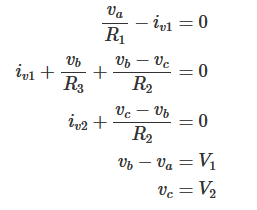
\includegraphics[width=.2\textwidth,scale=1]{Equations}
        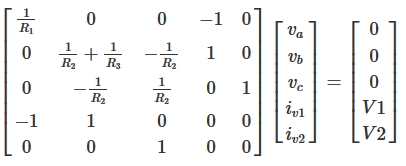
\includegraphics[width=50mm,scale=1]{Matrix}
        \caption{Process of conversion of equations into a matrix \cite{nodeanalysis}}
        \label{fig:figure3}
    \end{figure}

    \pagebreak
    \subsection{Characteristics of the MNA matrix}
    All circuits when presented in matrix for, will always result in the form:
    $$Ax = b$$
    In the given example matrix\footnote{Red highlight is $[N\times N]$ and matrix is $[(N+M)\times (N+M)]$ where 
    $N$ is the nodes in the circuit and $M$ is the number of independent sources.}:
    \begin{figure}[h]
        \centering
        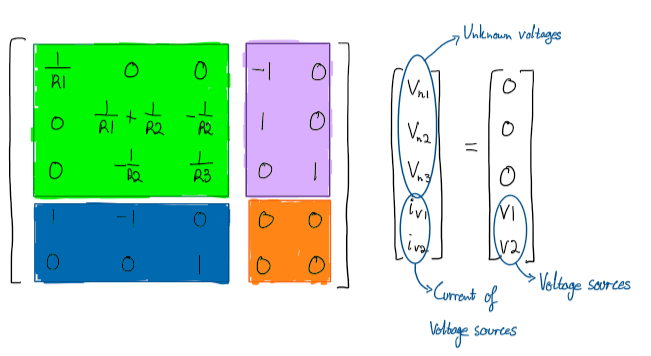
\includegraphics[width=50mm,scale=1]{Highlighted matrix}
        \caption{Characteristics of $Ax = b$}
        \label{}
    \end{figure}
    \par
    The following characteristics will always hold:
    \begin{itemize}
        \item Matrix A
        \begin{itemize}
            \item The highlighted part is size $[N \times N]$ and contains values of passive elements
            \item The main diagonal is positive values only. Non-diagonal values are either 0 or negative.
            \item If an element is grounded, it will appear along diagonal. 
        \end{itemize}
        \item Matrix $x$: Matrix of unknown quantities:
        \begin{itemize}
            \item General dimension: $[(N+M)\times1]$
            \item Top $N$ elements are simply node voltages
            \item Bottom $M$ elements are the currents related to voltage sources\footnote{Dependent current and voltage sources have not been considered yet}
        \end{itemize}
        \item Matrix $b$: Matrix containing known quantities:
        \begin{itemize}
            \item General dimension: $[(N+M)\times1]$
            \item Top $N$ elements are either 0 or sum of independent current sources
            \item Bottom $M$ elements are independent voltage sources
        \end{itemize}
    \end{itemize}
    Solution is found by:
    $$x = A^{-1}b$$
    \vfill
    \subsection{Notations}
    The naming notation is the following:\cite{nodeanalysis}.
    \begin{itemize}
        \item Ground is labelled \textbf{Node 0}
        \item Each node is given a label starting from 1 to $N$ 
        \item Node voltage name: $v\_N$
        \item Current through V sources: $i\_VoltageSourceName$
        \item Independent voltage sources: $vname$
        \item Independent voltage sources: $iname$
    \end{itemize}

    \pagebreak
    \section{General Algorithm design for MNA}
    Matrices need that need to be generated:
    \begin{itemize}
        \item $A$ 
        \item $x$ 
        \item $b$
    \end{itemize}
    \subsection{$A$ matrix}
    The $A$ matrix has dimension $[(M+N) \times (M+N)]$ and is combined from four smaller matrices: $A_a$, $A_b$, $A_c$ and $A_d$ \cite{nodeanalysis}.
    \par
    The respective matrices are defined as:
    \begin{itemize}
        \item $A_a$: $n \times n$ matrix - Passive element connections
        \item $A_b$: $n \times m$ matrix - Voltage source connections 
        \item $A_c$: $m \times n$ matrix - Similar to matrix $A_b$
        \item $A_d$: $m \times m$ matrix - 0 if independent sources are considered
    \end{itemize}

    \subsubsection{$A_a$ matrix}
    \begin{itemize}
        \item Size $N\times N$
        \item Each element in diagonal matrix is the conductance of each element connected to respective node
        \item Elements not on diagonal are negative conductances of the element connected to respective node.
        \item Non-grounded element will have one entry.
        \item Non-grounded element will have four entries.
    \end{itemize}
    For example:
    \begin{figure}[htp]
        \centering
        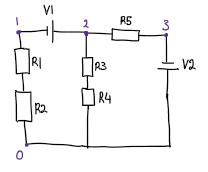
\includegraphics[width=.2\textwidth,scale=1]{Circuit2}
        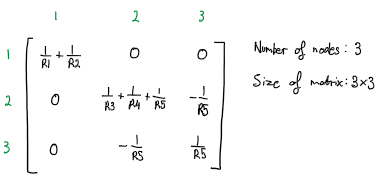
\includegraphics[width=50mm,scale=1]{Matrix2}
        \caption{The relationship between diagonal and non-diagonal elements}
        \label{fig:figure3}
    \end{figure}
    \pagebreak
    \subsubsection{$A_b$ matrix}
    \begin{itemize}
        \item Size $N\times M$
        \item Only 1, 0 and -1 entries
        \item Direction of voltage source matter. Negative terminal is -1 and positive terminal is 1.
        \item A grounded voltage source will have one entry.
        \item Non-grounded voltage source will have two entries.
    \end{itemize}
    The positive terminal of V1 in the above circuit is connected to node 2 as indicated in matrix element $[1, 2]$ where $1$ is $Vi$ and 2 is the node the terminal is connected to.
    \par
    For example: 
    \begin{figure}[htp]
        \centering
        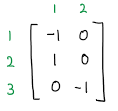
\includegraphics[width=25mm,scale=0.25]{Matrix3}
        \caption{Matrix showing the direction of voltage sources}
        \label{fig:figure3}
    \end{figure}

    \subsubsection{$A_c$ matrix}
    \begin{itemize}
        \item Size $M\times N$
        \item \textbf{Usually the transpose of $A_b$}
        \begin{itemize}
            \item Not the case if dependent sources are involved.
        \end{itemize}
    \end{itemize}
   
    \subsubsection{$A_d$ matrix}
    \begin{itemize}
        \item Size $M\times M$
        \item Usually composed of 0
        \begin{itemize}
            \item Not the case if dependent sources are involved.
        \end{itemize}
    \end{itemize}
    \vfill
    \pagebreak

    \subsection{$x$ matrix}
    The $x$ matrix has dimension $[N \times M]$ and is combined from two smaller matrices: $x_a$ and $x_b$. 
    \par
    The respective matrices are defined as:
    \begin{itemize}
        \item $x_a$: $N \times 1$ - Unknown node voltages
        \item $x_b$: $M \times 1$ - Unknown currents through voltage sources
    \end{itemize}
    \subsubsection{$x_a$ matrix}
    The naming follows the notation set out earlier. \par 
    \textbf{There is no entry for Ground (Node 0)}.
    \begin{figure}[htp]
        \centering
        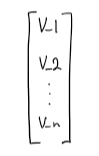
\includegraphics[width=20mm,scale=0.25]{Matrix4}
        \caption{General notation of the $x_a$ matrix}
        \label{fig:figure3}
    \end{figure}
    \subsubsection{$x_b$ matrix}
    Corresponds to the number of voltage sources. Example given in Figure 2.
    \subsection{$b$ matrix}
    This matrix has dimension $[(N \times M)) \times 1]$ and contains the independent current and voltage sources.
    
    The matrix is composed of two matrices: $b_a$ and $b_b$:
    \begin{itemize}
        \item $b_a$: $N \times 1$ Either 0 or the sum of independent current sources.
        \item $b_b$: $M \times 1$ Values of independent voltage sources.
    \end{itemize}
    \pagebreak

    \section{Support for $C$ and $L$ elements}
    Adding support for reactive elements, the code in requires modifications and additions. Before that is possible, 
    further insight is required as to how $C$ and $L$ can be represented in MNA. This will allow us to identify what functions 
    need to be implemented and how to best incorporate it into the existing codebase.\par
    \subsection{Theory behind capacitor and inductor}
    Capacitors can be seen as a current source defined by the equation:
    \begin{center}
        $i_{(t)} = C\frac{dv}{dt}$ \par
    \end{center}
    Inductors can be seen as a voltage source defined by the equation:
    \begin{center}
        $v_{(t)} = L\frac{di}{dt}$ \par
    \end{center}
    \subsection{Changes required}
    \begin{itemize}
        \item New parameter $\omega$ needs to be defined
        \begin{itemize}
            \item Default 0 if no frequency value entered
            \begin{itemize}
                \item Capacitor appears as a open circuit
                \item Inductor appears as a short circuit
            \end{itemize}
        \end{itemize}
        \item Data structures need to be changed to support complex numbers
    \end{itemize}


   
    \pagebreak

    \section{Dependent sources}
    \subsection{Voltage Controlled Current Source (VCVS)}
    \pagebreak

    \section{The use of Eigen library}
    Eigen is a linear algebra library used in the C++ environment. For our project, we chose to implement 
    Eigen functions to handle the matrix related operations such as finding inverse matrix 
    and matrix initialisation.
    \par
    The design decision is reached when we considered
    the disadvantages of writing our own matrix libraries, mainly:
    \begin{itemize}
        \item \textbf{Poor performance} unless significant time is spent optimising which will come at the cost of
        neglecting other aspects of the project.
        \item \textbf{Buggy code} unless significant time is spent considering edge cases, going back to first point.
    \end{itemize}
    By using an established library like Eigen, we have several advantages:
    \begin{itemize}
        \item \textbf{Up to date and well tested code}
        \item \textbf{Dynamic matrices and optimised structures} this will allow us to easily accomodate  
        optimisations in other aspects of the software package.
        \item \textbf{Very optimised code}

    \end{itemize}
    \pagebreak

    \section{Implementation}
    \begin{figure}[htp]
        \centering
        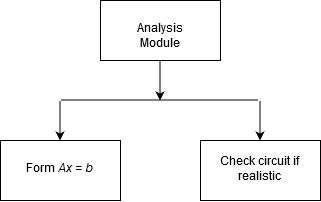
\includegraphics[width=80mm,scale=1]{Analysis breakdown}
        \caption{\textit{Analysis module} breakdown}
        \label{fig:figure3}
    \end{figure}

    \subsection{Analysis}
    \begin{lstlisting}[language=C++]
        Analysis
        {
            Get N and M
            Initialise matrices
            Form Ax = b
            Check circuit semantics
            Find inverse of A
            Solve for x
        }
    \end{lstlisting}

    \subsubsection{FormMatrix}
    \begin{lstlisting}[language=C++]
        Analysis(vector<CirElement>)
        {
            For loop over entire circuit vector
            {
                Identify component type

                Case: R,C or L
                {
                    Check if grounded
                    Insert in A matrix [Diagonal and non-diagonal]
                }
                
                Case: I
                {
                    Check if grounded
                    Insert in b matrix
                }

                Case: V
                {
                    Check if grounded
                    Add 1 or -1 in A matrix             
                    Insert in b matrix
                    Insert in x matrix [Unknown values are 0]            
                }
            }
            return matrix x;
        }
    \end{lstlisting}
    \subsubsection{SemanticCheck}
    \begin{lstlisting}[language=C++]
        SemanticCheck(vector<CirElement>)
        {
            Check if node are at least paired [Ignore node 0]
        }
    \end{lstlisting}
    
    \pagebreak

    \section{Version history}
    \subsection{Version 1.0}
    
    \pagebreak
    \section{Miscellaneous}



    \pagebreak
    \printbibliography[title={References}]
\end{document}